\chapter{Research Description}
\label{sec:researchdesc} 

\section{Introduction}
\label{sec:introduction}

\section{Background of the Study}
\label{sec:backgroundstudy}

% What is NA Quantification and its applications ? %
Quantification of nucleic acids is a developing research field in molecular biology for the detection and quantification expression levels of genes \cite{Huggett2015_PCR_NGS}. These molecules are found in deoxyribonucleic acid (DNA) and ribonucleic acid (RNA), which carries genetic information and is used as biomarkers for the detection of diseases. Additionally, along with the rise of bioinformatics tools, quantification methods are also utilized in rare mutation detection, copy number variation detection, single-cell gene and microRNA expression analysis, and next-generation sequencing \cite{Quan2018}. Outside the scope of molecular biology, its application has also found its way in forensic research \cite{Whale2013}, medical diagnosis, environmental monitoring, and food safety analysis \cite{Cao2017}.

% TODO : Brief history of dPCR (3 sentences ) %
% TODO : What is the difference of qPCR with dPCR (2 sentences) %

% How to Quantify NA Quantification with (dPRC) ? %
To be able to determine the concentration of target nucleic acid, detection is naturally a pre-requisite. There are, however, nucleic acid of interests that have very low concentrations to the point that it becomes undetectable in existing detection technologies. This problem is solved by amplifying the nucleic acid sequences using Polymerase Chain Reaction (PCR), a widely-used method for nucleic acid amplification since its invention in the 1980s \cite{Cao2017}. PCR can multiply specific nucleic acid sequences in DNA or RNA from low concentrations to millions of copies. This method exposes the nucleic acid sequences mixed with chemical components in a series of 20 to 40 temperature cycles. In each cycle, PCR doubles the nucleic acid molecule; theoretically producing \(2^n\) molecules after \(n\) cycles \cite{Quan2018}.

After PCR amplification, absolute nucleic acid quantification is achieved using digital Polymerase Chain Reaction (dPCR) technique. This equally divides the nucleic acid samples into thousands of partitions; each of these partitions is evaluated as either off or on, or in this context, labeled as positive or negative, hence the term "digital" \cite{Cao2017}.

% What are the advantages of dPCR? %
Since the earliest published dPCR experiment from 1988 (\citeauthor{Saiki1988}), the advances of nanofluidic technology in biomedical instruments have continuously pushed the limits of dPCR. An increasing number of researchers have found dPCR to be reaching, and even outperforming, the precision, sensitivity, and reproducibility of qPCR, which is the gold standard for molecular quantification \cite{Chen2018, Persson2018, Taylor2017, Arvia2017, Blaya2016, Jones2016, Sanders2011}. The nature of dPCR allows it to standardize quantitation as opposed to qPCR's use of a reference curve, resistant to inhibition, and less negatively influenced by the target sequence variability \cite{Sedlak2014}. The unraveling superiority of dPCR makes it a necessity for research experiments that require intensive accuracy, such as the certification or stability studies of reference materials.


% - GMO - Because of regulation of cultivation and trade of GMOs in several countries, there is pressure for their accurate detection and quantification. Today, DNA-based approaches are more popular for this purpose than protein-based methods, and real-time quantitative PCR (qPCR) is still the gold standard in GMO analytics. However, digital PCR (dPCR) offers several advantages over qPCR, making this new technique appealing also for GMO analysis. (Demeke) %
% - circRnucleic acid - Diagnostics based on circulating circular RNA (circRNA) is an emerging field for noninvasive molecular diagnosis, owing to the stable circular structure of circRNA. However, CircRNA remains stable in the promptly separated serum/plasma within 24 h and is a promising candidate for biomarker research. In addition, because the concentration of circRNA will be affected if the clotted blood and EDTA blood are not centrifuged promptly, samples should be handed in a timely manner to reduce the hematocyte-derived varia- tion. (Chen, DF) %

% What are the current challenges in dPCR experiments? %
Despite the optimistic performance of dPCR, several challenges are met before being able to reach the optimal results from dPCR. One of the final steps in dPCR is the threshold determination that separates the endpoint fluorescence of the dPCR assay into positives and negatives. The determination of this threshold is not constant for different DNA samples and unclear for assays that produce ambiguous readouts \cite{Trypsteen2015}.

An important aspect in positioning the threshold is the presence of noise features in the data. Poor quality dPCR assays adds to the ambiguity of fluorescence signals that contribute to the difficulty of threshold determination. Due to the emerging demand for dPCR data analysis, \citeA{Lievens2016} has determined a set of method performance criteria to assess the quality of a dPCR assay run. Their following criteria aims to measure the efficiency of the separation between positive and negative droplets: (i) there should only be two fluorescence populations, or in other terms, a single amplification product; (ii) there should be a good separation between positives and negatives measured in peak resolution; and (iii) there should be very minimal amounts of intermediate fluorescence, which is also termed as ‘rain’. The factors affecting these noise characteristics are further explored in the succeeding sections. 

In the case of three or more fluorescence populations, this formation may be attributed to a group of inhibited targets that had varying amplification efficiency as the other targets. This may also be the case of high presence of intermediate fluorescences for unoptimized assays \cite{Lievens2016}.

"Rain" is the term used in several studies to describe droplets that emits a fluorescence intensity settling in between the positive and negative populations \cite{Lievens2016, Trypsteen2015, Witte2016, Dreo2014, Brink2018, Attali2016}. Figures \ref{fig:plate1cru} and \ref{fig:plate1tc1507} demonstrates two different DNA targets with the former showing a visually clearer distinction of the positive and negative population than the latter, of which is possessing multiple rain droplets. The data used in these figures are sourced from the publicly available dataset from the study of \shortciteA{Lievens2016}.


% What are the consequences for analyzing poor quality data? %
Poor quality dPCR assays negatively limit the level of sensitivity and accuracy it may reach. Among the consequence of unoptimized dPCR assays is droplet misclassification, which may lead to serious incorrect conclusions.

The primary problem in misclassification lies in 'rain' droplets; these are partitions that emits an intermediate fluorescence signal that is difficult to classify as positive or negative. Figures \ref{fig:plate1cru} and \ref{fig:plate1tc1507} demonstrates two different DNA targets with the former showing a visually clearer distinction of the positive and negative population than the latter, of which is possessing multiple rain droplets. The data used in these figures are sourced from the publicly available dataset from the study of \shortciteA{Lievens2016}. 

\begin{figure}[h]
    \centering
    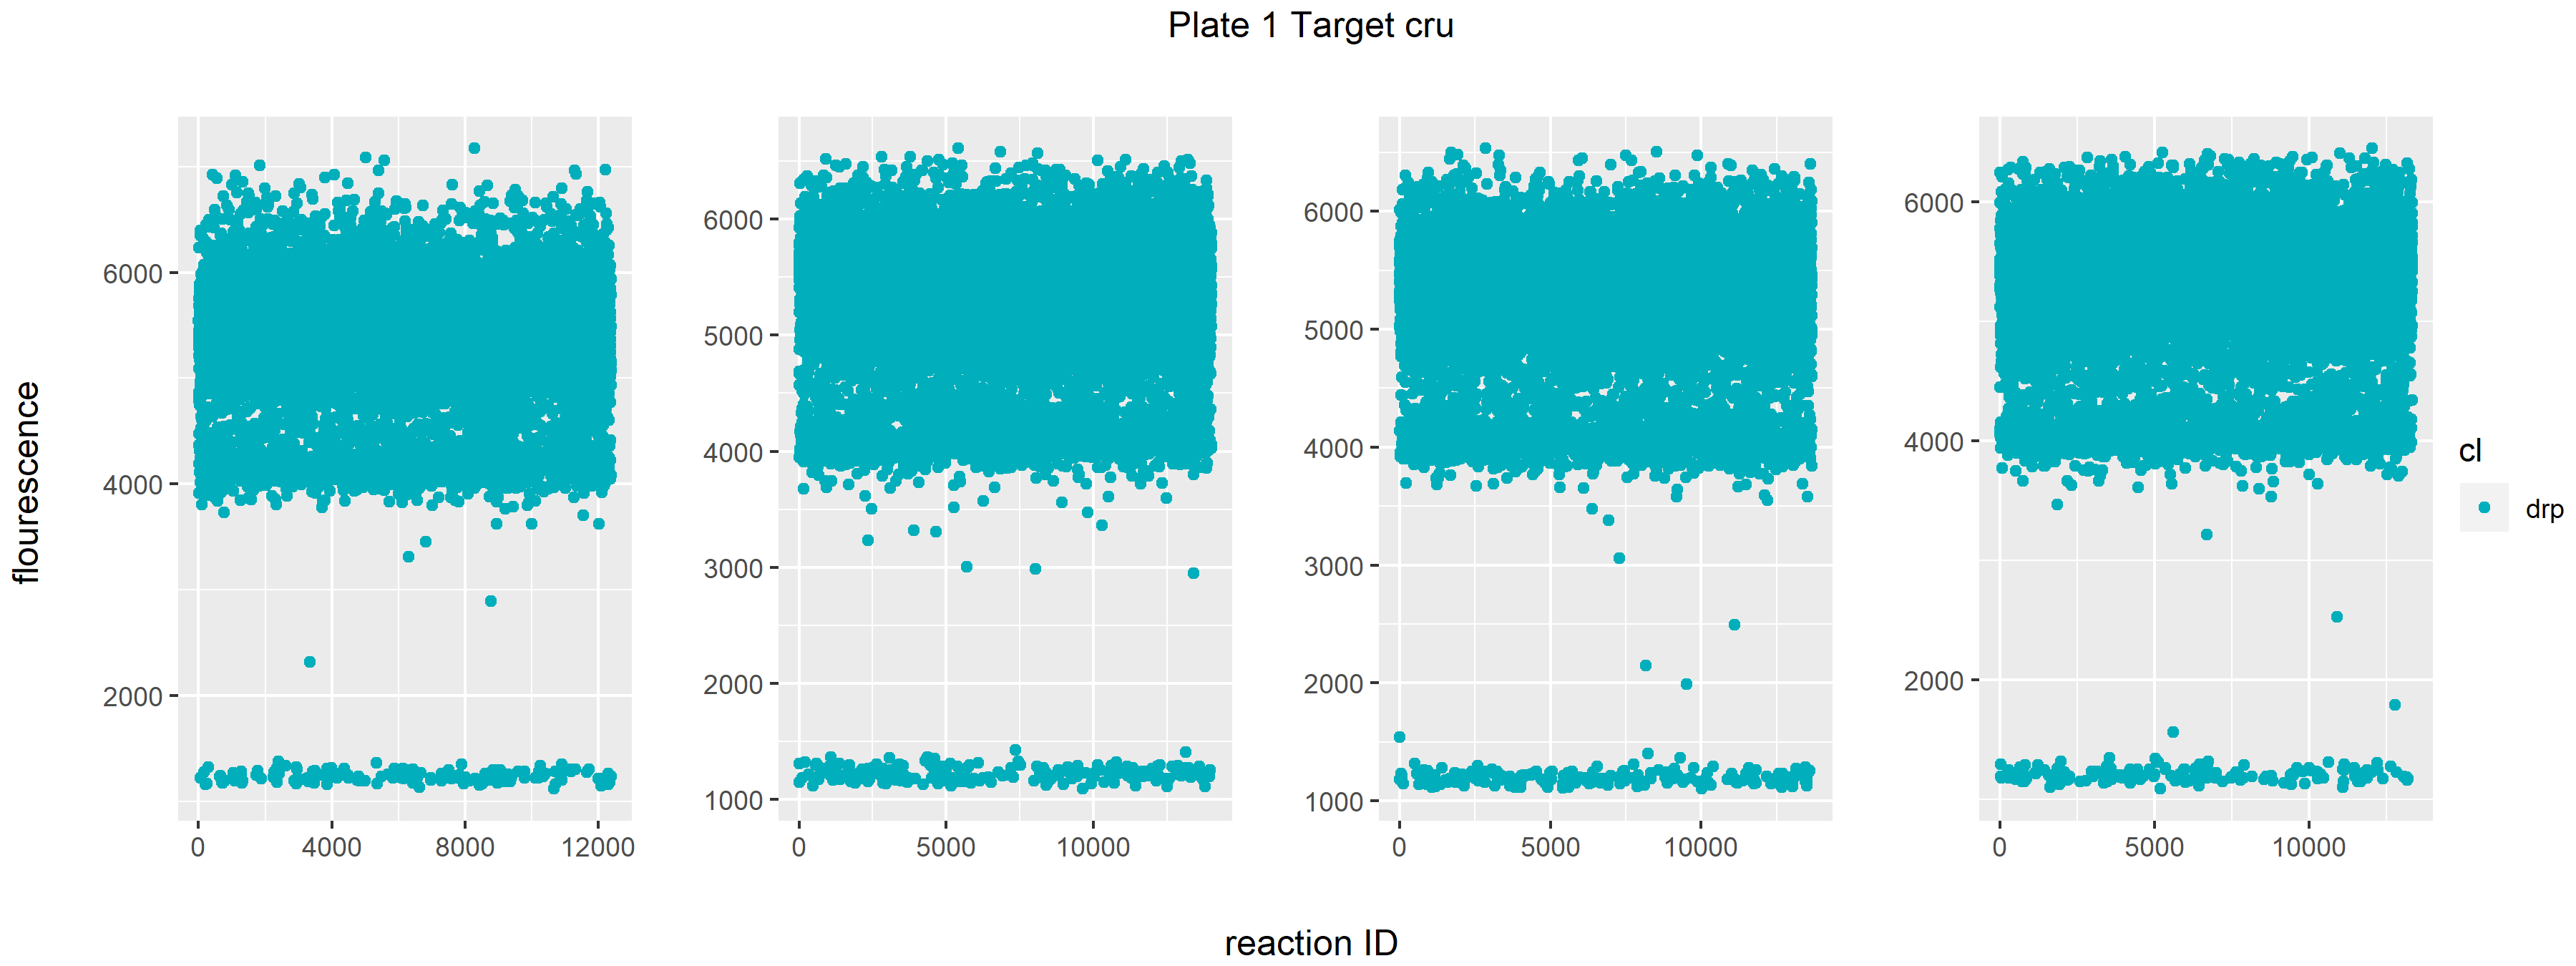
\includegraphics[max size={\textwidth}{\textheight}]{Plate 1 Target cru.png}
    \caption{Fluorescence readings of 4 repititions of DNA target cru}
        \label{fig:plate1cru}
\end{figure}

\begin{figure}[h]
    \centering
    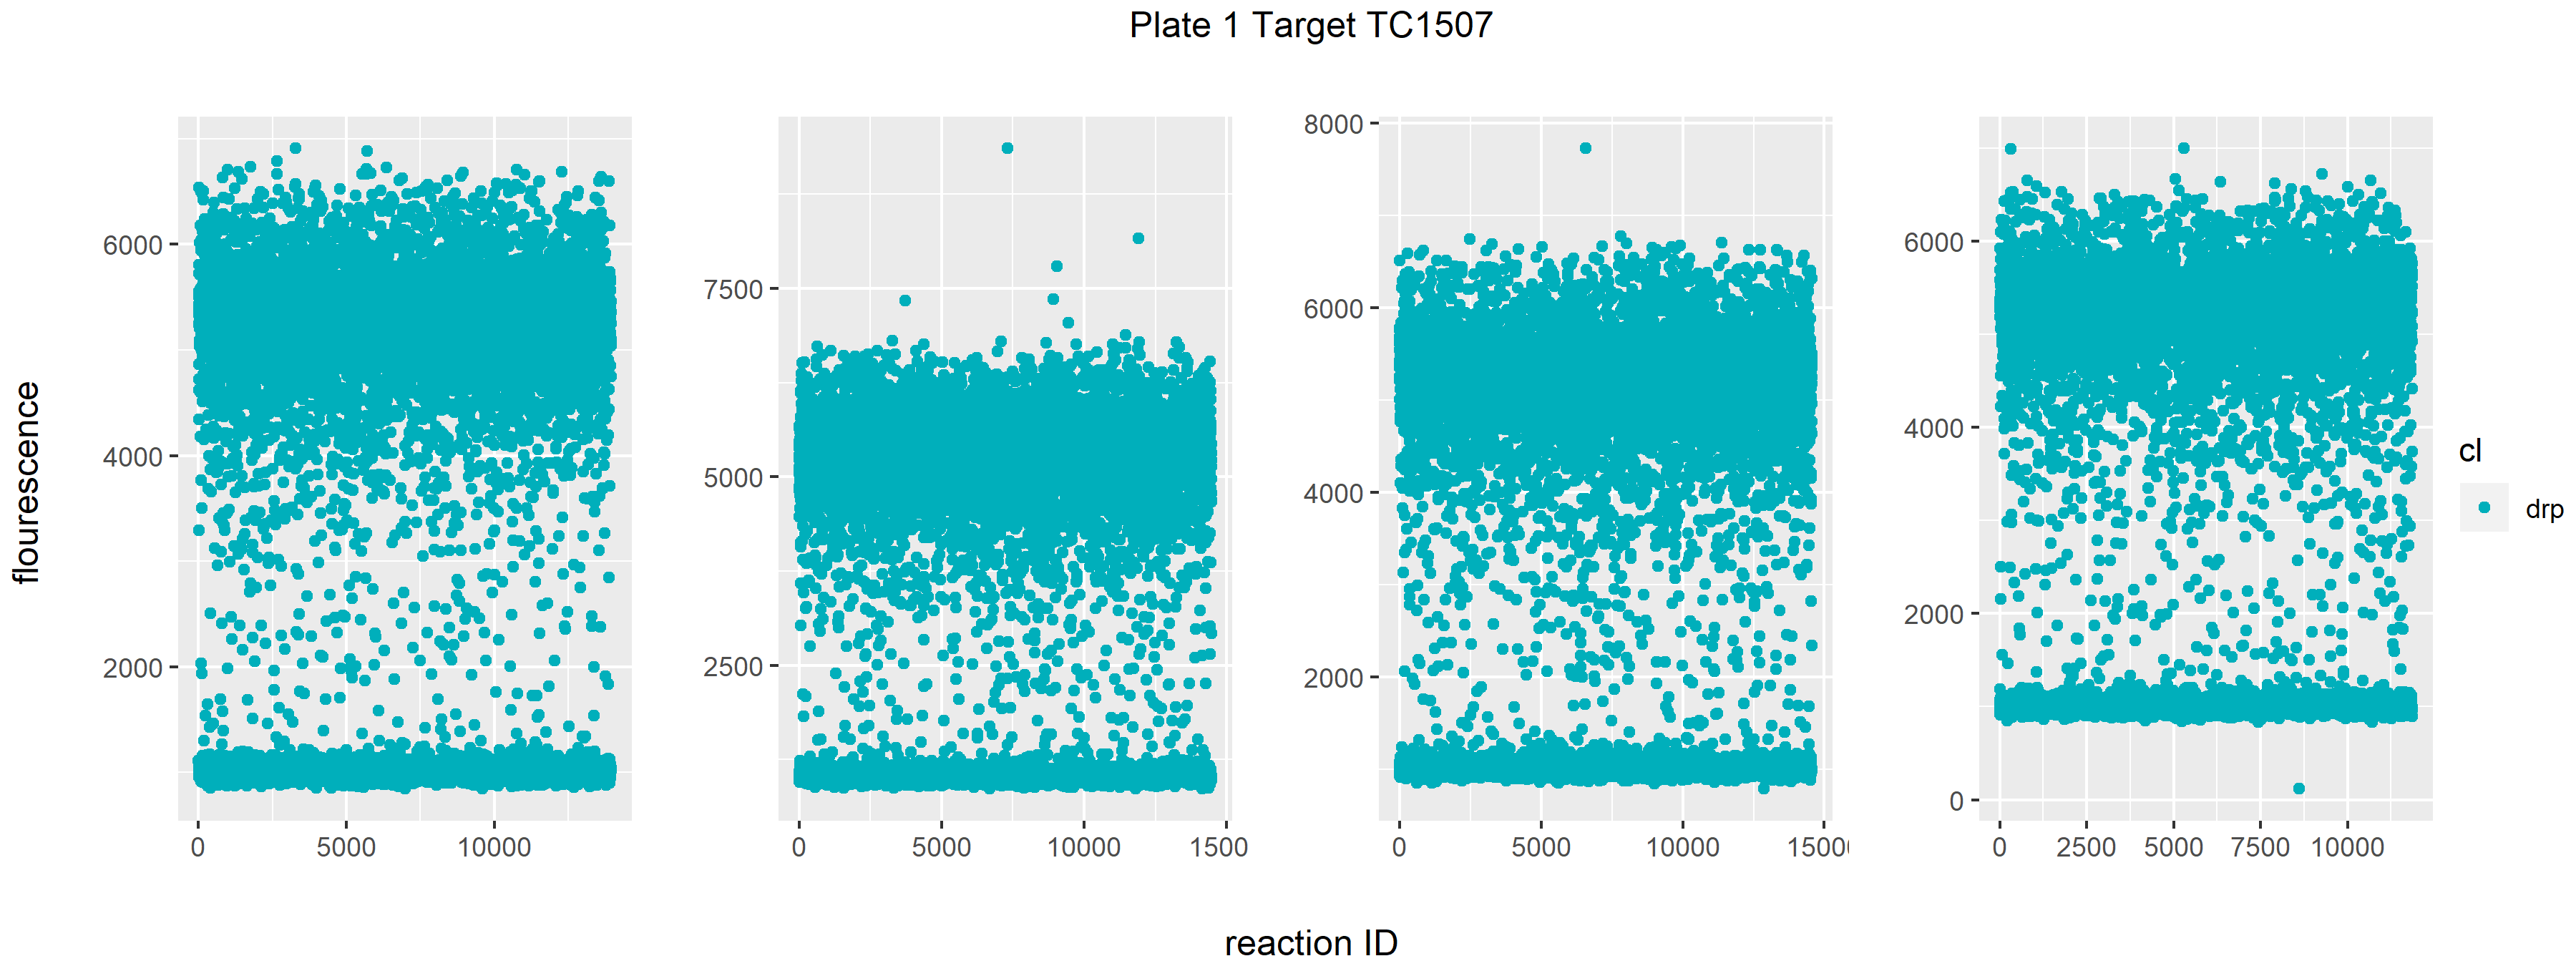
\includegraphics[max size={\textwidth}{\textheight}]{Plate 1 Target TC1507.png}
    \caption{Fluorescence readings of 4 repititions of DNA target TC1507}
        \label{fig:plate1tc1507}
\end{figure}

The estimate for DNA target concentration highly depends on the positive and negative classifications. For experiments with low copy DNA targets, the focus is on maximizing the sensitivity of the test for these very small number of positive droplets. Low sensitivity translates to failure in detecting lower concentrations. 

For assays with large differences in the distance between the two fluorescence groups (positive and negative droplets), most quantification tools estimate the target concentrations with high sensitivity. As exhibited in an optimized assay experiment of E. amylovora \cite{Dreo2014}, slight differences of thresholds calculated from different tools had little effect on the final estimated concentration. However, for R. solanacearum, which is observed to manifest false-positive signals in qPCR experiments, produces unsatisfactory analytical sensitivity of the concentration estimates. 

The danger of false rates due to misclassification is expounded at the clinical level, where false rates lead to the misdiagnosis of patients \cite{Tzonev2018}. One such case is the prenatal screening test for Down Syndrome; this test is expected to mostly result in normal pregnancies. However, even for a small FPR, many pregnancies are still falsely reported as positive for Down Syndrome. False negatives also risk the overall health of the patient that truly possesses the genetic disorder.

% What are the factors that cause these noise %
The whole dPCR workflow introduces multiple entry points for error and sources of variations, each of which is the possible source of such noise. The dPCR workflow, as illustrated in \figref{fig:dpcrWorkflow}, is usually a sequential procedure of extracting the sample from an organism, concocting the sample with several chemical components into a reaction mix, distributing the reaction mix to equal partitions, amplifying and detecting the target molecules using PCR, and the concentration is then finally estimated using a Poisson correction factor. In \cite{Jacobs2014}, it was emphasized that every step of the dPCR workflow inevitably allows for the introduction of different sources of variation. These variance components within the dPCR workflow are shown in \figref{fig:dpcrWorkflow}. 

\begin{figure}[h]
    \centering
    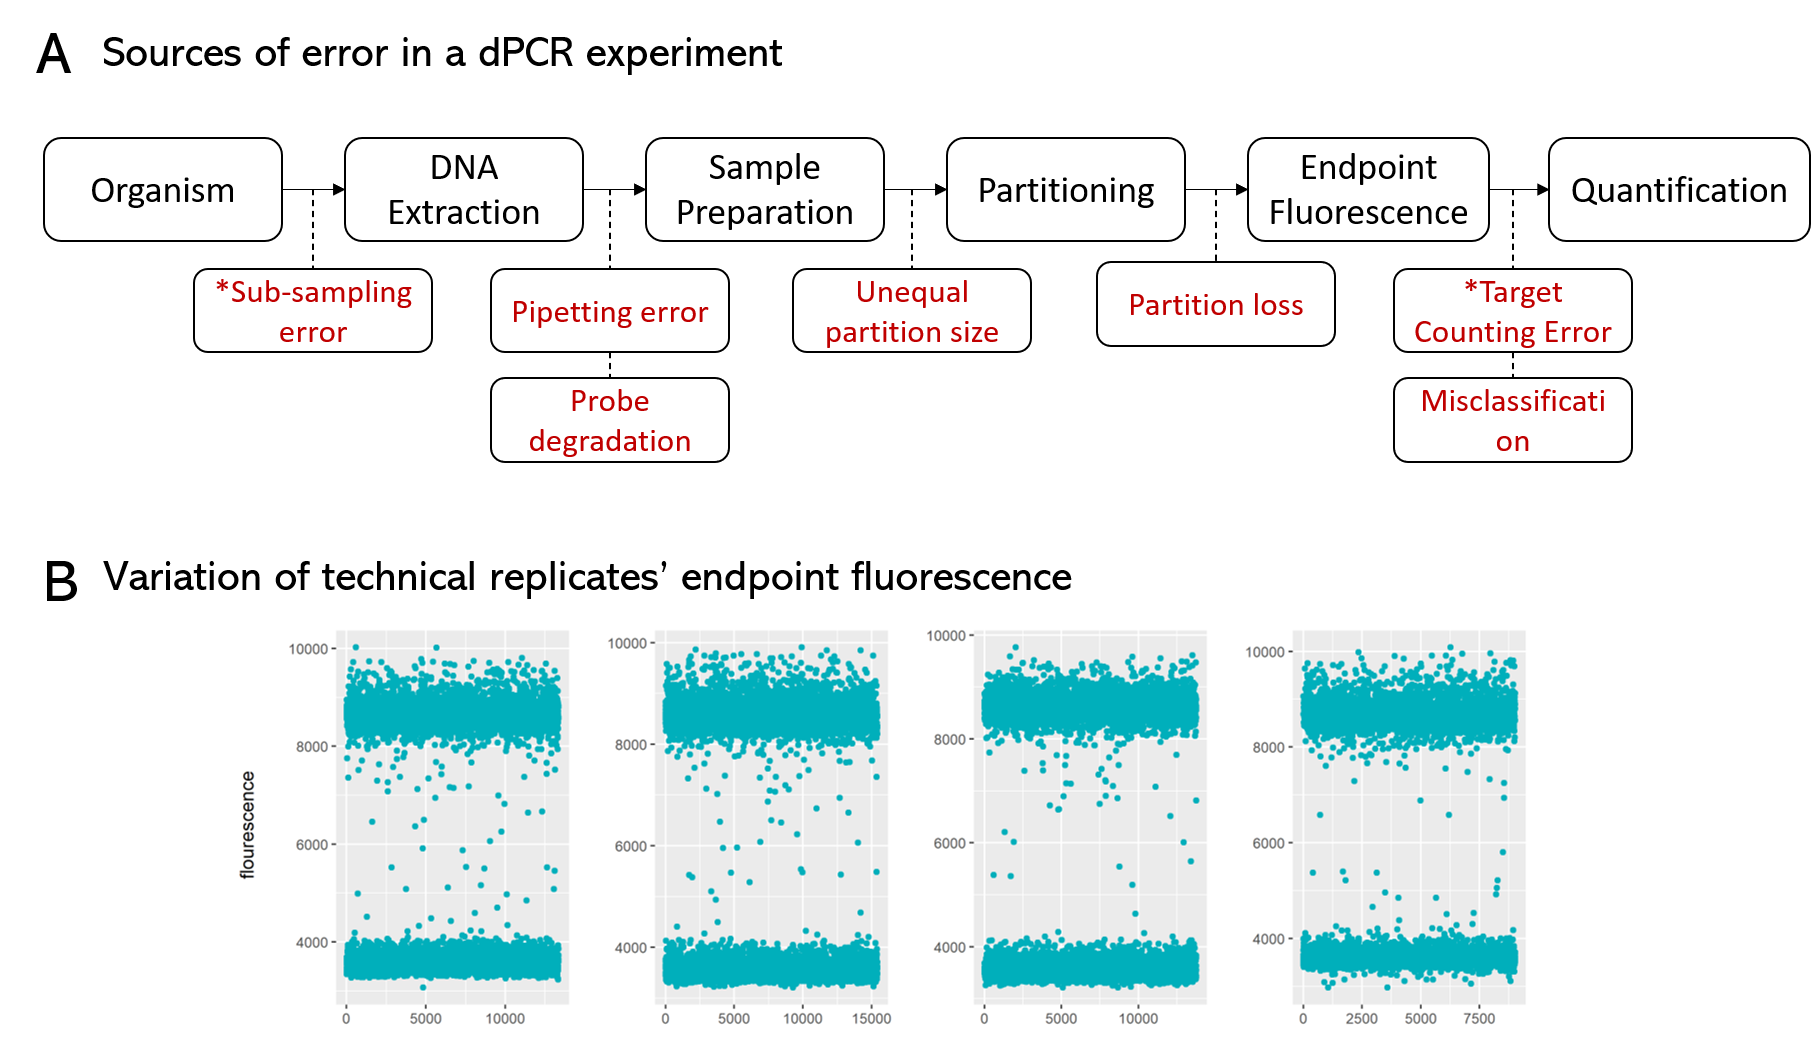
\includegraphics[max size={\textwidth}{\textheight}]{dpcrWorkflow.png}
    \caption[Sources of variation in the dPCR workflow]%
    {Sources of variation in the dPCR workflow- (A) Multiple sources of error can be introduced for each step in the dPCR workflow. Items with '*' indicate sampling error). (B) In effect, sample replicates obtained from the same organism will inevitably have variation in its fluorescence readouts. }
        \label{fig:dpcrWorkflow}
\end{figure}

% Physical variations %
Different dPCR systems do not share a common default setting and thermal profiles. Each one is a factor that has to be optimized depending on the target molecule. Increasing the number of cycles has shown to affect the amplification of dPCR droplets that separates the two populations better \cite{Koppel2015}. Temperature gradients are frequently performed to find the most favorable setting to reduce rain \cite{Gerdes2016}. However, the optimized parameters to improve the quality of a target's dPCR assay may not work for another target. As shown in the experiment of \shortciteA{Witte2016}, parameters that increased the efficiency for prfA did not work for \(\Delta\)prfA.

Besides controllable settings, different dPCR platforms also have been revealed to deviate from its claimed volume \cite{Pinheiro2012,Dong2015,Corbisier2015,Dagata2016,Kosir2017}. These discrepancies have been observed in the Bio-Rad QX100/QX200 platforms and the RainDrop platform. Unequal partition volumes may produce suboptimal PCR amplification that contributes to increased rain droplets.

% Biological and Chemical variations % 
Preparing the reaction mix is a delicate process that strictly requires the accuracy of the pipetting volume; and yet, technical variation still occurs that results in pipetting errors. In addition to physical variation, chemical and biological factors play a role in the dPCR assay quality, such as target sequence variation, concentration of polymerase, MgCI2, dNTPs, and primers \cite{Koppel2015, Kramer2001}, dye or probe quencher \cite{Witte2016}, and the fluorophore used \cite{Gerdes2016}, inhibition, delayed reactions, primer depletion, and other biological factors \cite{Jacobs2014}.

% Sampling variations %
Sampling variation stems from the fact that only a small sample of the organism is extracted; and although there is an expected number of target molecules per liters of a sample, drawing equally sized samples will result in different target molecules that are more or less near the average. \shortciteA{Tzonev2018} demonstrates the number of target molecules that can be drawn from extraction is distributed as Poisson. Besides the sampling error, samples may also exhibit imperfections, and thus have inhibited amplification. 

Each variance component accumulates to the bias and variance of the final estimated target concentration, and thus, this gives rise to the importance of providing solutions that would increase precision in every step. To increase the sensitivity and specificity of the estimate, the misclassification of droplet partition should be minimized as much as possible. A high presence of false-negative droplets reduces sensitivity, while specificity is lowered for high false-positive counts. 

% What can be done to reduce the noise indicated above? %
The identification of the factor directly influencing the noise present is very difficult to pinpoint. In case of failure to optimize the design parameters, other hands-on approaches may be taken, such as running a qPCR experiment, running PCR solution in gel electrophoresis, or performing dilution series in the cost of additional labor. However, preparing replicate samples are prone to pipetting and operator errors. On the other hand, the problem may also be alleviated using statistical approaches. Even in unoptimized assays, \citeA{Demeke2018} were still able to produce reliable results upon the automatic threshold set that enabled for the increased repeatability. Reliable automated threshold systems eliminate the operator bias from manually adjusting the threshold. When dealing with rain, some researchers exclude it in the final droplet counts \cite{Jones2014}, but this option is said to produce underestimated concentrations if rain were actually suboptimal PCR reactions; instead, the threshold algorithm should be improved \cite{Trypsteen2015}. Some researchers. In the case of droplet volume variability, correction-factor must be taken to improve the agreement of estimates  \cite{Demeke2018}.  For unresolved noise features, it is important to take this uncertainty into account and include it in the final estimate error.

% A statistical approach is proposed in this study. %
Expounding further on the automated threshold setting approach, such algorithms can be improved and should be robust to baseline shifts, rain droplets, multiple populations, and poor separation of populations. The baseline fluorescence of the negative population has been observed, but even the popularly used QuantaSoft systems do not take this into account \cite{Trypsteen2015}. Thus, discrepancies may occur in the number of positive droplets.

The threshold setting problem may be seen as a droplet classification problem. Reducing the misclassification while being robust to different data characteristics increases the reliability of the system. There are currently areas of improvement as automatic systems are said to be not yet the best option for the cases of abundant intermediate fluorescence \cite{Demeke2018}. Ideally, this system should be able to provide precise estimates regardless of dPCR assay quality, and thus, reducing the negative impact from compromising quality with time. As noted by several studies, dPCR assay quality is often traded with time. Even when an optimal setting is determined, it may be time-consuming to run the optimal parameters \cite{Witte2016}, such as when increasing cycles \cite{Lievens2016}, thermal profile variations of thermocyclers \cite{Young2008}. 



\section{Statement of the Problem}
\label{sec:statementprob}

This thesis aims to classify dPCR droplet partitions into positive or negative by exploring Model-Based clustering with Expectation Maximization. The specific objectives of this study are to:
\begin{enumerate}
    \item Find initialization parameters and fit G-component mixture densities on dPCR droplet fluorescence intensities.
    \item Utilize EM clustered droplets to provide precise quantification estimates for DNA samples with varying amounts of “noise” and concentration.
    \item Evaluate and compare the precision and bias of the estimates amongst the existing classification methods. 
\end{enumerate}

\section{Significance of the Study}
\label{sec:significancestudy}
Quantification of target concentrations for pathogenic bacteria, gene expression of diseases, cancer diagnostic, and other health-related applications strongly demand estimators with high sensitivity and precision, as lives are put to risk for false-positives. A modern approach to DNA and RNA target quantification is through the dPCR method. In one of the steps of the dPCR workflow, the classification of droplet fluorescence still has areas of improvement. 

The most prominent problem in classification lies in experiments exhibiting a high frequency of rain, or intermediate fluorescence values. These are experiments that have not yet been optimized. As different DNA target samples exhibit distinct structures \cite{Lievens2016}, an optimized setup for one DNA target may not be applicable for other targets. Additionally, for samples with low concentration, the total count of detected positive droplets dramatically changes the final concentration estimate, due to the greater impact of false positives in the proportion of detected over the number of true positives. The following are some tools and methodologies proposed for droplet classification: Quantasoft propriety software, definetherain \cite{Jones2014}, manual global threshold \cite{Dreo2014}, cloudy \cite{Lievens2016}, and Umbrella \cite{Jacobs2017}. Most of the aforementioned droplet classifying tools rely strongly on how representative reference samples are. According to \citeA{Dreo2014}, such approaches are sensitive to significant shifts in amplitude for previously unobserved factors, such as cross-reactions or the influence of inhibitors.

In an attempt to prevent the problem of representation, this study will explore the feasibility of estimating target concentrations without a reference sample. Additionally, multimodal distributions are considered as not to restrict the possibility of multiple fluorescence populations. The method used in this paper uses the concept of iterative parameter estimation from Cloudy and the model-based clustering for the droplet classification from Umbrella. This is both achieved using Expectation-Maximization algorithm. The significance of the study will be useful in quantifying precise concentrations in targets that have not yet been optimized for dPCR experiments and also for quantifying targets of low concentrations. 

\section{Scope and Limitations}
\label{sec:significance}
This study solely relied on publicly available fluorescence datasets from published research papers. Only two were found and will be used for statistical analysis, namely from \shortciteA{Lievens2016} and \shortciteA{Jones2014}. The former dataset contains twelve DNA targets from food and feed samples ran on nine different settings by controlling for experimental factors; the latter dataset is a serial dilution of the Albumin DNA ranging from \(10^0\) to \(10^5\) copies. 

The droplet classification method in this study uses model-based clustering, or the use of finite mixture models to perform clustering. However, the identification of the distribution of the mixture densities will be dependent on the observed available dataset. As a consequence of the limited dataset, the paper's methodology described here needs more study for other experimental setting and nucleic acid targets.

Lastly, statistical results presented may lack biological explanations which could be useful for explaining the variances of the droplet fluorescence. Such information may be utilized to further improve the estimation process.